\section{Background}\label{sec:background}

\subsection{The GFA Format}\label{subsec:gfa-format}

GFA is a line-oriented text format for sequence graphs~\cite{gfaspec}. Biologically, a graph node represents a DNA sequence segment (often shared by many individuals), edges represent allowed adjacencies between segments, and traversals represent assembled sequences or haplotypes as ordered walks through those segments.

The node record is \textbf{S} (segment), which stores a segment identifier and its DNA sequence.
Edge records include \textbf{L} (link), \textbf{J} (jump), and \textbf{C} (containment): \textbf{L} connects oriented segments (with overlap information), \textbf{J} represents long-range connections or gaps, and \textbf{C} represents containment/nesting relationships.
Traversal records are \textbf{P} (path) and \textbf{W} (walk). Both describe an ordered, orientation-aware route through nodes, which reconstructs a longer biological sequence from graph segments. \textbf{P} is a general named traversal (often a contig or reference path), while \textbf{W} (GFA~1.1) represents haplotype walks with explicit sample, haplotype, and coordinate metadata.
\textbf{H} (header) stores file-level metadata, and optional \texttt{TAG:TYPE:VALUE} fields extend records with additional annotations.
Figure~\ref{fig:gfa_visualization} shows a visualization of a GFA file using Bandage~\cite{Wick2015Bandage}.

\begin{figure}[t]
    \centering
    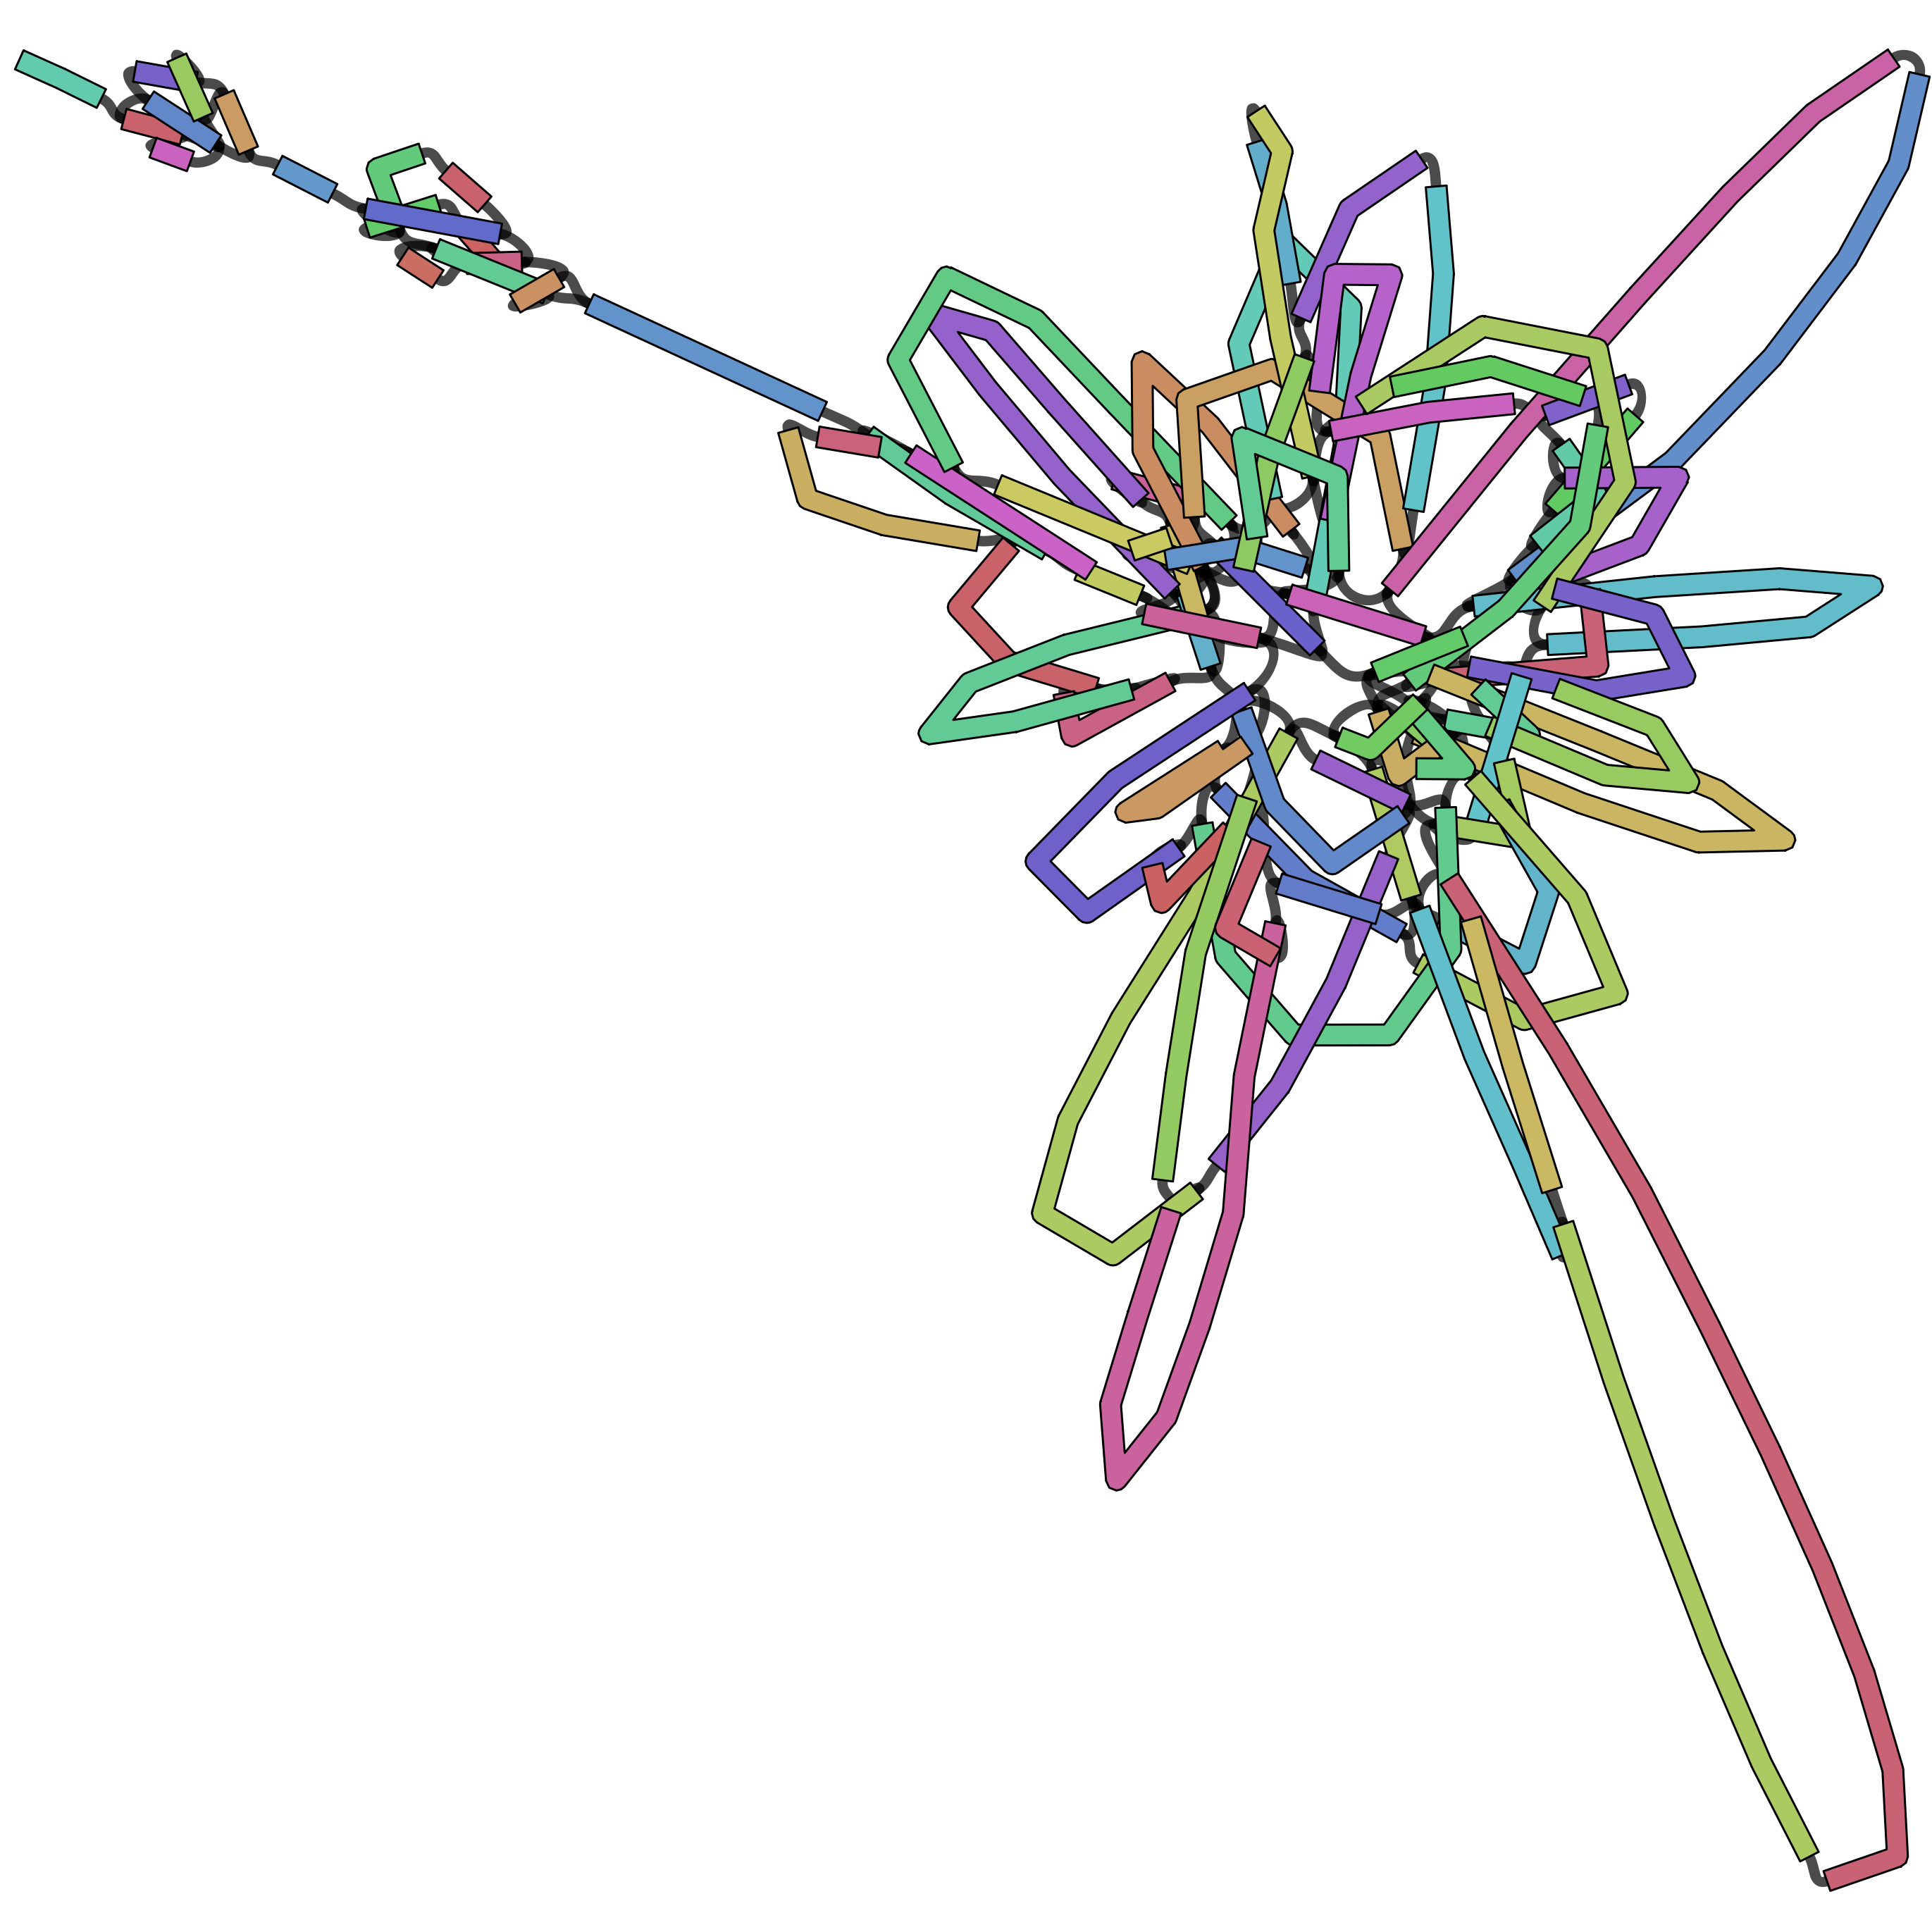
\includegraphics[width=\columnwidth]{GFA_visualization.png}
    \caption{Assembly graph in GFA format, visualized with Bandage~\cite{Wick2015Bandage}. Colored elements denote sequence segments (nodes; S records). Black connections indicate edges between oriented segments, represented by L (link), J (jump), or C (containment) records. Any valid traversal through connected segments corresponds to a P (path) or W (walk) record.}
    \label{fig:gfa_visualization}
\end{figure}

\subsection{The Scalability Challenge}\label{subsec:scalability}

GFA is widely used in graph-based genomics, including assembly graphs, pangenome construction, and downstream analysis. In pangenome graphs, shared sequence is merged into common nodes and variants form alternate branches. HPRC releases have grown from tens to hundreds of haplotypes and continue to expand~\cite{wang2022human,hprc_timeline}. Many downstream tools operate directly on GFA graphs, so these large files create both memory pressure during analysis and substantial storage overhead. At this scale, GFA becomes a systems bottleneck rather than only a storage nuisance.

As highlighted in Section~\ref{sec:intro}, real pangenome GFA files already reach very large sizes. The core scaling mechanism is structural: topology (S/L/J/C records) grows sublinearly as haplotypes are added, but traversal records (P/W) grow near-linearly because each haplotype walk is materialized explicitly. Since human haplotypes are highly similar, these long traversal streams contain substantial repeated node-ID substrings across samples. At even larger population sequencing scales, this growth will continue, pushing GFA datasets beyond hundreds gigabytes into multi-terabyte regimes. In practice, pipelines also produce many intermediate GFAs (per chromosome, per version, and per region), further amplifying storage and transfer costs.

Generic compressors cannot exploit most of this redundancy. Their small sliding windows miss long-range similarity across chromosome-length paths, so compression ratio remains limited for GFA files.

\subsection{Existing Compression Approaches}\label{subsec:existing}

Because generic compressors miss long-range path redundancy, specialized GFA compressors are needed. Other genomic compression families are also not a direct fit: read/alignment formats such as BAM/CRAM~\cite{li2009sequence, bonfield2022cram} target mapped reads rather than graph interchange files, and FASTQ compressors such as GPUFastQLZ~\cite{yang2024gpufastqlz} target linear sequence collections rather than graph topology and traversal semantics. For GFA graphs, compression must remain fully lossless to preserve graph structure and metadata while still exploiting cross-haplotype traversal redundancy.
Two graph-native approaches are GBZ and sqz.

GBZ uses Graph-Based Burrows–Wheeler Transform (GBWT)~\cite{siren2020haplotype, siren2021pangenomics} to store large collections of similar paths efficiently. This design is effective for large pangenomes with many similar haplotypes.
Its weaknesses are practical. Performance can degrade in highly collapsed repetitive regions, and compression ratio is less favorable on small graphs. Because GBWT construction is global, GBZ also does not naturally support incremental updates (e.g., appending new haplotypes) without rebuilding the index. In addition, GBZ does not preserve full GFA record semantics, like optional fields.

sqz keeps a text workflow and applies a heap-based BPE grammar design~\cite{zouhar2023formal} to path records. It repeatedly selects frequent adjacent 2-mers and replaces them with new rules.
The main limitations are speed and memory cost. After each new rule, sqz updates frequencies of affected neighboring pairs through adjacency-list bookkeeping, which makes each rule-creation step expensive in practice. This sequential dependency also limits parallelization, because each next substitution depends on the current global pair statistics. Similar to GBZ, sqz does not preserve full optional-field information, so it is not truly lossless for complete GFA records.
